\chapter{几何阿贝尔类域论}\label{L15}\lecturedate{2020/04/08}\sourcepage{125}
本讲讨论$n=1$时的几何Langlands对应。这一情形相当简单，也已经得到充分理解。

设$X$为$\F_q$或$\C$上的光滑射影曲线。回忆，Langlands对应的几何重述断言存在以下单向映射：
\begin{figure}[H]\centering\begin{equation}\tag{0.1}\label{L15eq01}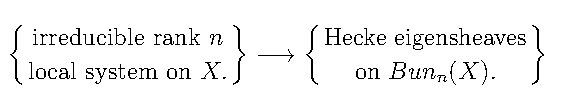
\includegraphics[width=0.4657\paperwidth]{images/L15-p125-correspondence.pdf}\end{equation}\end{figure}
设$E_\sigma$为$X$上对应于表示$\sigma:\widehat\pi_1(X)\to\GL_n(\overline{\Q}_\ell)$的$\overline{\Q}_\ell$局部系统。若对每个$i=1,\ldots,n$，均存在同构
\begin{equation}\tag{0.2}\label{L15eq02}T^i(\mathcal F_\sigma)\cong\bigwedge^iE_\sigma\boxtimes\mathcal F_\sigma,\end{equation}
则称$\mathcal F_\sigma\in D_c^b(\operatorname{Bun}_n(X))$为相对于$\sigma$的Hecke特征层，其中$\bigwedge^i$表示第$i$次外幂。

现在令$n=1$。首先，将线丛模叠$\operatorname{Bun}_1(X)$的标量自同构刚性化\znoteplain{线丛模叠的每个对象都带有 $\C^\times$ 的标量自同构，因此它是 $\operatorname{Pic}(X)$ 上的 $\C^\times$-gerbe，而不是概形。刚性化就是把这些标量自同构固定下来（等价于把该 gerbe 平凡化），从而得到 Picard 概形。同样的说法在§3 用于局部系统：刚性化的一维局部系统指附带一个固定同构 $\psi:\mathcal A_L|_0\cong\overline{\Q}_\ell$，即指定了基点处纤维的一个标架。（上下文推断，无外部依据）}，得到$X$的Picard概形$\operatorname{Pic}(X)$。其次，只需考虑Hecke算子$T^1$。于是\eqref{L15eq02}中的Hecke特征层条件简化为
\begin{equation}\tag{0.3}\label{L15eq03}T^1(\mathcal F_\sigma)\cong E_\sigma\boxtimes\mathcal F_\sigma.\end{equation}
我们将看到，$X$上的一维$\ell$进局部系统$E_\sigma$对应的Hecke特征对象$\mathcal F_\sigma$实际上是一个层，而非多项复形。此外，在$n=1$时，这些Hecke特征层可以由内在性质定义，而不必先涉及$X$上的$\ell$进局部系统；\eqref{L15eq01}的映射此时为双射。
\sourcepage{126}
\section{\texorpdfstring{$n=1$时的Hecke算子$T^1$}{n=1时的Hecke算子T¹}}\label{L15S1}
一个标准事实是：若$F$为可分闭域，则$\widehat\pi_1(\mathbb P_F^n,\overline x)=1$。可以假设曲线$X$在几何上不是$\mathbb P^1$，因而$g(X)\ge1$。
\originalnumber{1}
\begin{lemma}\label{L15S1O1}
设$X$为$k$上的光滑射影几何连通曲线，且$g(X)\ge1$。则$X$上不同的$k$-点$x_1,x_2$不可能线性等价，即
\[\OO_X(x_1)\cong\OO_X(x_2)\quad\Longleftrightarrow\quad x_1=x_2.\]
\end{lemma}
\begin{proof}
若$x_1,x_2$不同却线性等价，则存在$f\in K(X)$，满足$\operatorname{div}(f)=x_1-x_2$，特别地，$f(x_1)=0$、$f(x_2)=\infty$。有理函数$f$诱导态射$f:X\to\mathbb P^1$，其次数为一，因为零点除子恰为$x_1$。这与$g(X)\ge1$矛盾。
\end{proof}
回忆，第$i$个Hecke对应$\mathcal H^i$参数化四元组$(\mathcal M,\mathcal M',x,\beta:\mathcal M\hookrightarrow\mathcal M')$。当$n=1$时，只有第一个Hecke对应$\mathcal H^1$及以下三个映射：
\begin{figure}[H]\centering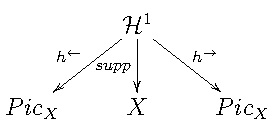
\includegraphics[width=0.2222\paperwidth]{images/L15-p126-Hecke.pdf}\end{figure}
它们满足下图所示的关系：
\begin{figure}[H]\centering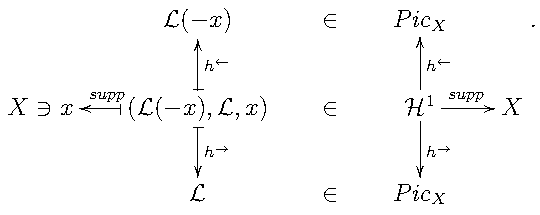
\includegraphics[width=0.4354\paperwidth]{images/L15-p126-maps.pdf}\end{figure}
由\eref{引理}{L15S1O1}及线丛修改的描述可知$\mathcal H^1\cong\operatorname{Pic}_X\times X$，且$\operatorname{supp}\times h^\rightarrow$为同构。Hecke函子写为
\[T^i(\mathcal K^\bullet)=(\operatorname{supp}\times h^\rightarrow)_*(h^\leftarrow)^{-1}(\mathcal K^\bullet)[i(n-i)].\]
因此，当$n=1$时，在以$\operatorname{supp}\times h^\rightarrow$识别两个空间后，$T^1$就是沿加点映射的逆像。更确切地说，以$\operatorname{Pic}_X^d$表示$\operatorname{Pic}_X$中参数化次数$d$线丛的分支，以$\mathcal F^d$表示层$\mathcal F$在该分支上的限制。
\sourcepage{127}
于是\eqref{L15eq03}中的Hecke特征层条件变为
\begin{equation}\tag{1.1}\label{L15eq11}m_X^{-1}(\mathcal F_\sigma^{d+1})\cong\mathcal F_\sigma^d\boxtimes L_\sigma,\end{equation}
其中$L_\sigma=E_\sigma$为表示$\sigma$所对应的局部系统，$m_X:\operatorname{Pic}_X^d\times X\to\operatorname{Pic}_X^{d+1}$为$(\mathcal L,x)\mapsto\mathcal L(x)$。
\section{曲线的对称幂}\label{L15S2}\idx{对称幂}\idx{Abel--Jacobi映射}
仍设$X$为域$k$上的光滑曲线。以$X^{(d)}$表示$X$的第$d$个对称幂\znote{$d$ 次对称幂首先是对向量空间定义的：$\operatorname{Sym}^dV$ 是 $d$ 重张量幂对 $\mathfrak S_d$ 置换作用的商，特征为零时可等同于不变张量。本讲的 $X^{(d)}$ 是同一构造在曲线上的几何版本：它参数化 $d$ 次有效除子 $x_1+\cdots+x_d$，即 $X^d$ 对 $\mathfrak S_d$ 的商。常见误解是「取商必生奇点」，但 $d\ge1$ 时 $X^{(d)}$ 仍然光滑（命题 2.2）。[来源：MathWorld 词条「Symmetric Power（对称幂）」，\url{https://mathworld.wolfram.com/SymmetricPower.html}（2026-11-14 访问）。]}，以$X^d$表示其$d$重乘积，则有仿射的商映射
\[\pi^d:X^d\longrightarrow X^{(d)}.\]
以$\mathfrak S_d$表示$d$次对称群，则$X^{(d)}\cong X^d/\!/\mathfrak S_d$。有一个自然的\textbf{Abel--Jacobi映射}\znote{经典情形下，$\operatorname{Div}^0(X)\to J(X)$ 由积分定义，Abel 定理说其核恰为主除子，于是它把除子的线性等价类实现为 Jacobian 簇中的点。$AJ_d$ 是它在 $d$ 次有效除子上的版本：$X^{(d)}$ 参数化 $d$ 次有效除子，$AJ_d$ 把它们送到 $\operatorname{Pic}_X^d$；由 Abel 定理，纤维正是同一线性等价类的全部有效除子，即完备线性系，故当 $d\ge2g-1$ 时纤维是射影空间（命题 2.5）。[来源：nLab 「Abel-Jacobi map」，\url{https://ncatlab.org/nlab/show/Abel-Jacobi+map}（Last revised 2023-06-09；2026-11-14 访问）。]}：
\begin{equation}\tag{2.1}\label{L15eq21}
AJ_d:X^{(d)}\longrightarrow\operatorname{Pic}_X^d,\qquad (x_1,\ldots,x_d)\longmapsto\OO_X(x_1+\cdots+x_d).
\end{equation}
\originalnumber{1}
\begin{note}[L15S2O1]
\eqref{L15eq21}中的$AJ_d$不仅是集合论映射，还是代数概形之间的态射，因为它来自相应函子之间的自然变换。
\end{note}
对两个正整数$d,e$，同构$X^d\times X^e\xrightarrow{\sim}X^{d+e}$诱导典范态射
\begin{equation}\tag{2.2}\label{L15eq22}\widetilde m_{d,e}:X^{(d)}\times X^{(e)}\longrightarrow X^{(d+e)}.\end{equation}
\originalnumber{2}
\begin{proposition}\label{L15S2O2}
当$d\ge1$时，$X^{(d)}$非奇异。
\end{proposition}
\begin{proof}
只需证明：对任意几何闭点$y\in X^{(d)}$，局部环$\OO_{X^{(d)},y}$的极大理想$\mathfrak m_y$可由不超过$d$个元素生成。由\eqref{L15eq22}，只需考虑$y=(x,x,\ldots,x)$的情形，其中$x\in X$。还可以将局部环换成其完备化$\widehat{\OO}_{X^{(d)},y}$。设$\widetilde y$为$y$在$X^d$中的原像，则
\[\widehat{\OO}_{X^{(d)},y}\cong(\widehat{\OO}_{X^d,\widetilde y})^{\mathfrak S_d}.\]
另一方面，在代数闭的剩余域上，$\widehat{\OO}_{X^d,\widetilde y}\cong\overline k[[t_1,\ldots,t_d]]$，且此同构将$\mathfrak m_{\widetilde y}$对应到$\langle t_1,\ldots,t_d\rangle$。
\sourcepage{128}
因而，在不变量环中有
\[\mathfrak m_y=\mathfrak m_{\widetilde y}\cap(\widehat{\OO}_{X^d,\widetilde y})^{\mathfrak S_d}\cong\langle\sigma_1,\ldots,\sigma_d\rangle,\]
其中$\sigma_j$为变量$t_1,\ldots,t_d$的第$j$个初等对称多项式。因此$\mathfrak m_y$可由$d$个元素生成，命题得证。
\end{proof}
设$L$为$X$上的一维$\ell$进局部系统。定义$L^{\boxtimes d}:=\bigotimes_{j=1}^d\operatorname{pr}_j^{-1}L$，其中$\operatorname{pr}_j:X^d\to X$为第$j$个因子的投影。于是$L^{\boxtimes d}$是$X^d$上的一维$\ell$进局部系统，带有$\mathfrak S_d$-线性化：对每个$\sigma\in\mathfrak S_d$及$(x_1,\ldots,x_d)\in X^d$，有同构
\[h_{(x_1,\ldots,x_d),\sigma}:\bigotimes_{j=1}^dL_{x_j}\xrightarrow{\sim}\bigotimes_{j=1}^dL_{x_{\sigma(j)}}.\]
\originalnumber{3}
\begin{proposition}\label{L15S2O3}
$L^{\boxtimes d}$下降为$X^{(d)}$上的一维$\ell$进局部系统$L^{(d)}$。
\end{proposition}
\begin{proof}
令$L^{(d)}:=(\pi_*L^{\boxtimes d})^{\mathfrak S_d}$，其中$\pi=\pi^d:X^d\to X^{(d)}$为商映射。只需证明$\pi^{-1}L^{(d)}\cong L^{\boxtimes d}$。注意，对态射$f:X\to Y$和$X$上的平展层$\mathcal F$，有自然映射$f^{-1}f_*\mathcal F\to\mathcal F$，因此得到
\begin{figure}[H]\centering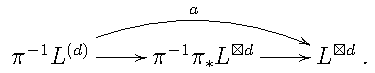
\includegraphics[width=0.3020\paperwidth]{images/L15-p128-descent.pdf}\end{figure}
由可构造层的真基变换性质，即\eref{定理}{L13S2O4}，映射$a:\pi^{-1}L^{(d)}\to L^{\boxtimes d}$在每个茎上均为同构，因而本身为同构。
\end{proof}
有以下交换图：
\begin{figure}[H]\centering\begin{equation}\tag{2.3}\label{L15eq23}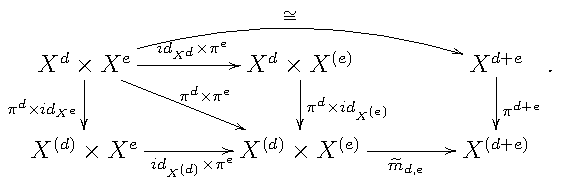
\includegraphics[width=0.4616\paperwidth]{images/L15-p128-symmetric.pdf}\end{equation}\end{figure}
\originalnumber{4}
\begin{proposition}\label{L15S2O4}
$\widetilde m_{d,e}^{-1}L^{(d+e)}\cong L^{(d)}\boxtimes L^{(e)}$。
\end{proposition}
\begin{proof}
由$X^d\times X^e\cong X^{d+e}$，有$L^{\boxtimes d}\boxtimes L^{\boxtimes e}\cong L^{\boxtimes(d+e)}$。由\eqref{L15eq23}，
\[\begin{aligned}
(\pi^d)^{-1}L^{(d)}\boxtimes(\pi^e)^{-1}L^{(e)}&\cong L^{\boxtimes(d+e)}\\
&\cong(\pi^{d+e})^{-1}L^{(d+e)}\\
&\cong(\pi^d\times\pi^e)^{-1}\widetilde m_{d,e}^{-1}L^{(d+e)}.
\end{aligned}\]
\sourcepage{129}
因此$\widetilde m_{d,e}^{-1}L^{(d+e)}\cong L^{(d)}\boxtimes L^{(e)}$，因为二者都是局部系统$L^{\boxtimes d}\boxtimes L^{\boxtimes e}$的相容下降。
\end{proof}
注意$X^{(1)}\cong X^1\cong X$，且$L^{(1)}\cong L$。因此$L^{(d)}$满足与\eqref{L15eq11}类似的Hecke特征层性质：
\begin{equation}\tag{2.4}\label{L15eq24}\widetilde m_{d,1}^{-1}L^{(d+1)}\cong L^{(d)}\boxtimes L.\end{equation}
由Riemann--Roch定理可以得到以下命题。
\originalnumber{5}
\begin{proposition}\label{L15S2O5}
设$g=g(X)\ge1$。若$d\ge2g-1$，则\eqref{L15eq21}中的Abel--Jacobi映射$AJ_d$为真满射，其在几何点$\Spec\Omega\to\operatorname{Pic}_X^d$处的几何纤维同构于射影空间$\mathbb P_\Omega^{d-g}$。
\end{proposition}
\section{Deligne的几何证明}\label{L15S3}\idx{几何阿贝尔类域论}\idx{乘法局部系统}
假设$X$有一个$k$-有理点$p$。我们要证明以下定理。
\originalnumber{1}
\begin{theorem}[Deligne]\label{L15S3O1}
以下两类对象的同构类一一对应：
\begin{figure}[H]\centering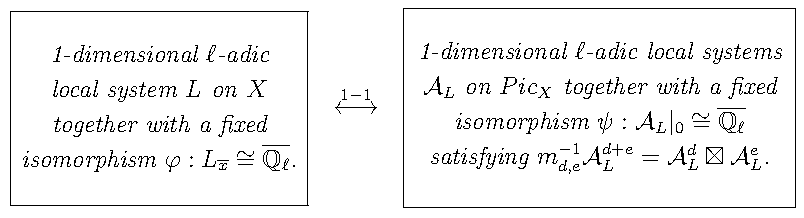
\includegraphics[width=0.6485\paperwidth]{images/L15-p129-Deligne.pdf}\end{figure}
这里$\mathcal A_L^d$为$\mathcal A_L$在分支$\operatorname{Pic}_X^d$上的限制，$m_{d,e}:\operatorname{Pic}_X^d\times\operatorname{Pic}_X^e\to\operatorname{Pic}_X^{d+e}$为线丛张量积诱导的自然映射。
\end{theorem}
\begin{proof}
给定一维$\ell$进局部系统$L$、几何点$x:\operatorname{Spec}\Omega\to X$\znoteplain{此处 $x$ 指几何点 $\operatorname{Spec}\Omega\to X$，与本节构造里用到的 $k$-有理点 $p$ 不是一类对象：$x$ 的剩余域是代数闭包 $\Omega$，只在取纤维 $L_{\bar x}$ 时出现；而 $p\in X(k)$ 才能用来把 $\mathcal A_L^d$ 沿 $dp$ 标架化。原书混用这两个记号，阅读时按 $L_{\bar x}$ 的下标理解即可。（上下文推断，无外部依据）}及固定同构$\varphi:L_{\overline x}\cong\overline{\Q}_\ell$，可以在$X^{(d)}$上构造一维$\ell$进局部系统$L^{(d)}$，它对应于Galois表示
\[\rho_{L^{(d)}}:\widehat\pi_1(X^{(d)})\longrightarrow\overline{\Q}_\ell^{\times}.\]
该表示经由阿贝尔化$\widehat\pi_1(X^{(d)})\to\widehat\pi_1^{\mathrm{ab}}(X^{(d)})$分解。
\sourcepage{130}
现在设$d\ge2g(X)-1$。由\eref{定理}{L10S3O1}及\eref{命题}{L15S2O5}，有正合列
\[\widehat\pi_1(\mathbb P_\Omega^{d-g},\overline x)\longrightarrow\widehat\pi_1(X^{(d)},\overline x)\longrightarrow\widehat\pi_1(\operatorname{Pic}_X^d,\overline{AJ_d(x)})\longrightarrow1.\]
由于$\widehat\pi_1(\mathbb P_\Omega^{d-g},\overline x)$平凡，$AJ_d$诱导基本群同构。因此$\widehat\pi_1(X^{(d)},\overline x)$的每个一维表示都诱导$\widehat\pi_1(\operatorname{Pic}_X^d,\overline{AJ_d(x)})$的唯一一维表示。于是，在$\operatorname{Pic}_X^d$上有唯一的一维$\ell$进局部系统$\mathcal A_L^d$，带有固定同构$\psi:\mathcal A_L^d|_{dp}\cong\overline{\Q}_\ell$，满足$AJ_d^{-1}\mathcal A_L^d\cong L^{(d)}$。

此外有下列交换图：
\begin{figure}[H]\centering\begin{equation}\tag{3.1}\label{L15eq31}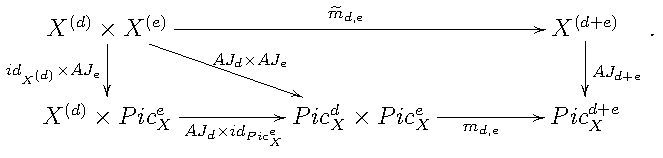
\includegraphics[width=0.5343\paperwidth]{images/L15-p130-tensor.pdf}\end{equation}\end{figure}
若$d,e\ge2g(X)-1$，由\eref{命题}{L15S2O4}可得$m_{d,e}^{-1}\mathcal A_L^{d+e}\cong\mathcal A_L^d\boxtimes\mathcal A_L^e$。

我们已经在$d\ge2g(X)-1$的分支$\operatorname{Pic}_X^d$上定义了$\mathcal A_L^d$，接下来要对所有$d\in\Z$构造它。利用\eqref{L15eq31}的交换图，令$e=1$，并选取$k$-有理点$p\in X$，有
\[\operatorname{Pic}_X^d\cong\{p\}\times\operatorname{Pic}_X^d\overset{i_p}{\hookrightarrow}X\times\operatorname{Pic}_X^d\xrightarrow{m_X}\operatorname{Pic}_X^{d+1}.\]
定义
\begin{equation}\tag{3.2}\label{L15eq32}\mathcal A_L^d:=i_p^{-1}m_X^{-1}(\mathcal A_L^{d+1})\otimes L_{\overline p}^{\vee}.\end{equation}
可以检验，以此方式定义的$\mathcal A_L$为$\operatorname{Pic}_X$上的一维$\ell$进局部系统，具有单位元处的固定同构$\psi:\mathcal A_L|_0\cong\overline{\Q}_\ell$，并满足$m_{d,e}^{-1}\mathcal A_L^{d+e}\cong\mathcal A_L^d\boxtimes\mathcal A_L^e$。

反过来，设$\mathcal A_L$为$\operatorname{Pic}_X$上刚性化的一维乘法$\ell$进局部系统。考虑Abel--Jacobi映射$AJ_1:X\to\operatorname{Pic}_X^1$。
\sourcepage{131}
其逆像$AJ_1^{-1}\mathcal A_L^1$为$X$上的一维$\ell$进局部系统；选取在$\overline p$处的标架后，它也具有刚性化。证明上述两个构造在同构类层面互为逆构造，留给读者。
\end{proof}
\originalnumber{2}
\begin{note}[L15S3O2]
若$k=\C$，则$\operatorname{Pic}_X^0$为$X$的Jacobian簇，且
\[\operatorname{Pic}_X^0\cong H^1(X,\OO_X)/H^1(X,\Z).\]
其平展基本群为阿贝尔群，且
\[\widehat\pi_1(\operatorname{Pic}_X^0)\cong\widehat{H_1(\operatorname{Pic}_X^0,\Z)}\cong\widehat{H_1(X,\Z)}\cong\widehat\pi_1^{\mathrm{ab}}(X).\]
这里帽号表示射有限完备化\znote{设 $N$ 取遍 $G$ 的有限指数正规子群，$G$ 的射有限完备化 $\widehat G$ 就是有限商 $G/N$ 在自然投影下的逆向极限；它是紧、Hausdorff、全不连通的拓扑群，而射有限群正是有限群的逆向极限。Galois 理论中的绝对 Galois 群与 étale 基本群天然是这种群，所以这里的「一维表示」须理解为取值于 $\overline{\Q}_\ell^\times$ 的连续同态，正因如此才能用有限层的同调来计算。[来源：nLab 「profinite group」，\url{https://ncatlab.org/nlab/show/profinite+group}（Last revised 2025-07-01；2026-11-14 访问）。]}。表示$\rho:\widehat\pi_1(X)\to\overline{\Q}_\ell^{\times}$经由$\widehat\pi_1(X)\to\widehat\pi_1^{\mathrm{ab}}(X)$分解。由Poincaré对偶，$H_1(X,\Z)$与$H^1(X,\Z)$典范对应。因此，$\widehat\pi_1(X)$的一维表示诱导$\widehat\pi_1(\operatorname{Pic}_X^0)$的唯一一维表示，可以将$L$对应到$\operatorname{Pic}_X^0$上的唯一局部系统$\mathcal A_L^0$。

再用递归公式\eqref{L15eq32}定义所有$d\le0$时的$\mathcal A_L^d$。当$d>0$时，有同构
\begin{figure}[H]\centering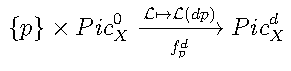
\includegraphics[width=0.2343\paperwidth]{images/L15-p131-translation.pdf}\end{figure}
并定义$\mathcal A_L^d\cong(f_p^d)_*(\mathcal A_L^0\otimes L_{\overline p}^{\otimes d})$。构造$L\leftrightarrow\mathcal A_L$实现了\eref{定理}{L15S3O1}中的一一对应。
\end{note}
\needspace{5\baselineskip}\section{第15讲参考文献}\label{L15S4}
\begin{references}
\refitem{L15bibT}{T} Péter Tóth, \emph{Geometric abelian class field theory}, Thesis for MD at Univ. Utrecht, available at \url{http://math.bu.edu/people/magner/Seminar/GCFTthesis.pdf}.
\refitem{L15bibL}{L} G. Laumon, \emph{Faisceaux Automorphes Lies aux Series Eisenstein}, In L. Clozel and J.S. Milne, editors, \emph{Automorphic Forms, Shimura Varieties and L-functions}, Academic Press, 1990.
\refitem{L15bibH}{H} J. Heinloth, \emph{Class field theory}, in \emph{Geometric Langlands Program winter school in Göttingen}, 2007.
\end{references}
